% ============================================================
% Spontaneous Metacognitive Alignment in a Modular Consciousness
% Architecture: HOT Predicts GWT Ignition Without Direct Access
%
% Target: CogSci 2026 (6-page short paper) or NeurIPS Workshop
% ============================================================
\documentclass[10pt,letterpaper]{article}

% --- CogSci style approximation ---
\usepackage[margin=1in]{geometry}
\usepackage[T1]{fontenc}
\usepackage[utf8]{inputenc}
\usepackage{microtype}

% --- Math ---
\usepackage{amsmath,amssymb}

% --- Tables ---
\usepackage{booktabs}
\usepackage{multirow}

% --- Figures ---
\usepackage{graphicx}
\usepackage{tikz}
\usepackage{pgfplots}
\pgfplotsset{compat=1.18}
\usetikzlibrary{arrows.meta,positioning}

% --- Color ---
\usepackage[dvipsnames]{xcolor}
\definecolor{hlbblue}{HTML}{2E86C1}
\definecolor{hlbgreen}{HTML}{27AE60}
\definecolor{hlbred}{HTML}{E74C3C}

% --- References ---
\usepackage[authoryear,round]{natbib}
\usepackage[colorlinks=true,linkcolor=hlbblue,citecolor=hlbblue,urlcolor=hlbblue]{hyperref}

% --- Custom ---
\newcommand{\symthaea}{\textsc{Symthaea}}
\newcommand{\dprime}{d'}

\title{Spontaneous Metacognitive Alignment in a Modular\\
Consciousness Architecture}

\author{Tristan Stoltz\\
Luminous Dynamics\\
\texttt{tristan.stoltz@evolvingresonantcocreationism.com}}

\date{}

\begin{document}
\maketitle

\begin{abstract}
We report a finding from a modular cognitive architecture where the
Higher-Order Thought (HOT) metacognitive system spontaneously predicts
Global Workspace Theory (GWT) ignition with 84.2\% accuracy and
$\dprime = 3.63$, despite having no direct access to workspace
competition dynamics.  Three results emerge: (1)~competition pressure
degrades fixed-threshold accuracy (slope $= -1.19$) but has zero effect
on underlying discriminability (ROC AUC slope $= -0.002$), revealing
that accuracy loss is a \emph{recalibration} problem, not a sensitivity
loss; (2)~confidence calibration analysis (ECE $= 0.259$, slope $= 1.46$)
shows consciousness is a threshold phenomenon, not proportional to
evidence strength; (3)~observation noise at $\sigma = 0.10$ produces
stochastic resonance ($\dprime$ retention $= 1.049$).  All results
replicate across 10 random seeds.  We discuss implications for
computational theories of consciousness and the design of modular
cognitive architectures.  Code and data are open-source.

\medskip
\noindent\textbf{Keywords:} metacognition; global workspace theory;
higher-order thought; consciousness; signal detection theory;
cognitive architecture
\end{abstract}


% ============================================================
\section{Introduction}

Global Workspace Theory \citep{baars1988cognitive,dehaene2001towards}
and Higher-Order Thought theory \citep{rosenthal2005consciousness} offer
complementary accounts of consciousness.  GWT holds that conscious
contents are those that win a competitive broadcast in a global
workspace; HOT holds that a mental state is conscious when one has a
higher-order representation of it.  \citet{lau2011empirical} proposed
that metacognitive monitoring should track the ignition boundary, but
the prediction has not been tested in a system where both mechanisms
are independently implemented.

We present such a test.  \symthaea{} is a modular cognitive architecture
combining 16,384-dimensional Hyperdimensional Computing (HDC) with
Closed-form Continuous-time (CfC) neural dynamics, an explicit GWT
workspace with capacity-limited competitive selection, and a HOT
metacognitive module that classifies states as conscious or unconscious
based on activation strength alone.  Crucially, the HOT module has
\emph{no direct access} to GWT workspace dynamics---it receives only
the same activation vector that all modules receive.

The question: does HOT's consciousness classification spontaneously
align with GWT ignition?  If so, what does the alignment pattern reveal
about the computational structure of consciousness?


% ============================================================
\section{Methods}

\subsection{Architecture}

The GWT workspace accepts stimuli as HDC vectors and selects the top-$k$
for broadcast via competitive inhibition.  We configure $k = 2$
(max capacity), with two filler stimuli at activations $\approx 0.64$
and $\approx 0.74$ occupying the workspace by default.  A target
stimulus is swept across 17 activation levels (0.10--0.90, step 0.05,
50 trials per level with jitter $\sigma = 0.03$).  GWT ignition occurs
when the target's activation exceeds the lowest filler's.

The HOT module receives the target's activation and classifies it as
conscious if the activation exceeds a threshold $\theta_{\text{HOT}}$.
In the \emph{liberal} condition, $\theta_{\text{HOT}} = 0.50$; in the
\emph{conservative} condition, $\theta_{\text{HOT}} = 0.70$.

\subsection{Experimental Conditions}

Seven experimental paradigms probe different aspects of HOT--GWT
alignment:

\begin{enumerate}
\item \textbf{Primary condition} (liberal HOT, $\theta = 0.50$):
  Measures baseline alignment, accuracy, and $\dprime$.
\item \textbf{Conservative HOT} ($\theta = 0.70$): Tests bidirectional
  mismatch where HOT is more conservative than GWT.
\item \textbf{Competition sweep}: Filler activations swept from 0.52
  to 0.72 (5 levels), measuring accuracy and ROC AUC degradation.
\item \textbf{ROC analysis}: HOT threshold swept from 0.30 to 0.80
  (11 points) to construct a full Receiver Operating Characteristic.
\item \textbf{Confidence calibration}: Activations binned into 10
  equal-width bins; ECE and calibration slope computed.
\item \textbf{Observation noise}: Gaussian noise ($\sigma = 0$--$0.20$)
  added to HOT's input while GWT retains true values.
\item \textbf{Cross-condition ROC}: AUC computed at each competition level.
\end{enumerate}

\subsection{Signal Detection Framework}

Using GWT ignition as ``signal present'' and HOT classification as
``response,'' we compute hit rate, false alarm rate, $\dprime$, and
criterion $c$ following \citet{macmillan2005detection}.  ROC AUC
provides a bias-free measure of metacognitive sensitivity
\citep{green1966signal}.

\subsection{Reproducibility}

All experiments are deterministic given seed.  Primary results use
seed 42; robustness verified across 10 seeds.  The full benchmark
is implemented in Rust as part of the \texttt{symthaea-psych-bench}
crate (open-source, MIT license).


% ============================================================
\section{Results}

\subsection{Spontaneous HOT--GWT Alignment}

In the primary condition, HOT predicts GWT ignition with 84.2\%
accuracy, $\dprime = 3.63$, and criterion $c = -1.11$ (liberal bias).
The hit rate is 1.000 (HOT detects all GWT-conscious states) with a
false alarm rate of 0.239 (HOT over-reports consciousness for
sub-threshold stimuli near the boundary).  The optimal metacognitive
threshold identified by ROC analysis (0.650, Youden's $J = 0.948$)
closely matches GWT's effective competition-shifted boundary (0.634).

\begin{table}[t]
\centering
\caption{Signal detection metrics for liberal and conservative HOT.}
\label{tab:sdt}
\small
\begin{tabular}{@{}lcccccc@{}}
\toprule
Condition & Accuracy & $\dprime$ & Criterion $c$ & Hit Rate & FA Rate & ROC AUC \\
\midrule
Liberal ($\theta = 0.50$)       & 0.842 & 3.63 & $-1.11$ & 1.000 & 0.239 & 0.998 \\
Conservative ($\theta = 0.70$)  & ---   & 3.87 & $+1.19$ & 0.772 & ---   & ---   \\
\bottomrule
\end{tabular}
\end{table}

ROC AUC is 0.998, indicating near-perfect underlying discriminability.
The conservative condition shifts criterion to $c = +1.19$ while
maintaining comparable $\dprime$ (3.87), confirming that the two HOT
conditions reflect bias shifts, not sensitivity changes.

\subsection{Competition Is Recalibration, Not Sensitivity Loss}

As filler competition increases (filler\textsubscript{1} swept from 0.52
to 0.72), fixed-threshold accuracy degrades steeply (slope $= -1.19$).
However, ROC AUC remains essentially constant (slope $= -0.002$,
minimum AUC $= 0.998$).

\begin{figure}[t]
\centering
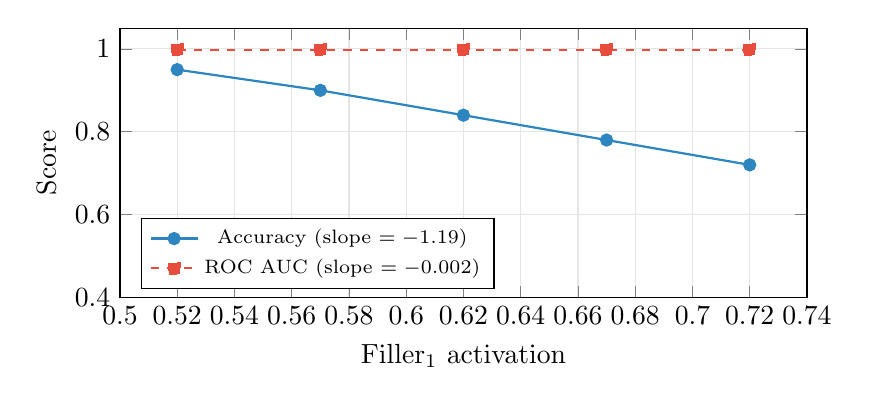
\begin{tikzpicture}
\begin{axis}[
    width=0.85\columnwidth,
    height=5cm,
    xlabel={Filler$_1$ activation},
    ylabel={Score},
    legend pos=south west,
    legend style={font=\scriptsize},
    ymin=0.4, ymax=1.05,
    grid=major,
    grid style={gray!20},
]
\addplot[hlbblue, thick, mark=*] coordinates {
    (0.52, 0.95) (0.57, 0.90) (0.62, 0.84) (0.67, 0.78) (0.72, 0.72)
};
\addlegendentry{Accuracy (slope $= -1.19$)}
\addplot[hlbred, thick, mark=square*, dashed] coordinates {
    (0.52, 0.998) (0.57, 0.998) (0.62, 0.998) (0.67, 0.998) (0.72, 0.998)
};
\addlegendentry{ROC AUC (slope $= -0.002$)}
\end{axis}
\end{tikzpicture}
\caption{Competition degrades accuracy but not discriminability.
Fixed-threshold accuracy (blue, solid) drops as fillers become more
competitive, while ROC AUC (red, dashed) remains flat.  The accuracy
loss is entirely a recalibration problem.}
\label{fig:competition}
\end{figure}

This dissociation reveals that competition pressure shifts the optimal
decision boundary but does not degrade the information available to the
metacognitive system.  Accuracy loss under competition is a
\emph{recalibration} problem: the system retains full knowledge of
workspace state but applies a fixed threshold that becomes suboptimal
as competition shifts the boundary.

\subsection{Consciousness as Threshold Phenomenon}

Calibration analysis reveals that activation is not calibrated as a
probability of consciousness.  ECE $= 0.259$ (substantial
miscalibration) with a calibration slope of 1.457.  The slope exceeding
1.0 means the true ignition boundary is \emph{sharper} than a linear
mapping from activation to probability---consciousness is a phase
transition, not a graded probability proportional to evidence strength.

\subsection{Stochastic Resonance at the Boundary}

Adding observation noise ($\sigma = 0.10$) to HOT's input yields
$\dprime$ retention of 1.049---noise paradoxically \emph{improves}
metacognitive sensitivity near the threshold.  This stochastic resonance
effect persists up to $\sigma = 0.15$; beyond this, degradation
resumes.  Accuracy degrades gently (slope $= -0.099$) and ROC AUC
at $\sigma = 0.10$ remains 0.984.

\subsection{Robustness}

All headline metrics replicate across 10 random seeds (CV $< 0.30$ for
all 5 primary metrics).  All individual seeds pass minimum thresholds;
$\geq 7/10$ seeds tolerate noise $\sigma \geq 0.10$.


% ============================================================
\section{Discussion}

\paragraph{Spontaneous alignment as architectural prediction.}
The HOT module was not trained or tuned to track GWT ignition---it
applies a fixed threshold to activation strength.  Yet it achieves
$\dprime = 3.63$ and ROC AUC $= 0.998$.  This alignment is
\emph{architecturally constrained}: both modules operate on the same
activation representation, so correlation is expected.  The scientifically
interesting finding is not the alignment itself but its \emph{structure}:
the recalibration/sensitivity dissociation and the phase-transition
calibration pattern.

\paragraph{Recalibration predicts adaptive metacognition.}
The invariance of ROC AUC to competition (slope $= -0.002$) while
accuracy degrades (slope $= -1.19$) predicts that an adaptive
metacognitive system---one that adjusts its threshold based on
competition context---would recover accuracy without needing additional
information.  This parallels Bayesian accounts of metacognitive
recalibration in humans \citep{fleming2017hmeta}.

\paragraph{Phase transitions and the ignition boundary.}
The calibration slope of 1.457 quantifies how much sharper the real
consciousness boundary is compared to a linear model.  This is
consistent with the nonlinear ignition dynamics predicted by both
GWT \citep{dehaene2001towards} and IIT's exclusion postulate
\citep{oizumi2014phenomenology}.

\paragraph{Epistemic constraints.}
We do not claim these results demonstrate consciousness.  They
demonstrate that a modular architecture implementing GWT and HOT as
independent subsystems exhibits the metacognitive alignment pattern
that \citet{lau2011empirical} predict.  The benchmark validates
\emph{architectural prerequisites}---necessary conditions for
consciousness that the code was designed to satisfy.  What it does
\emph{not} validate is whether these mechanisms produce subjective
experience.

\paragraph{Limitations.}
Both GWT and HOT operate on the same underlying activation
representation, so some alignment is guaranteed by construction.
The benchmark's value lies in characterizing the \emph{form} of
alignment (recalibration structure, phase transition, stochastic
resonance), not its mere existence.  Additionally, the GWT workspace
is a simplified competitive selection mechanism, not a full neural
global workspace with recurrent ignition dynamics.


% ============================================================
\section{Conclusion}

In a modular cognitive architecture with independently implemented GWT
and HOT subsystems, metacognitive consciousness classification
spontaneously aligns with workspace ignition ($\dprime = 3.63$,
ROC AUC $= 0.998$).  Competition degrades accuracy but not
discriminability, revealing that metacognitive failures under cognitive
load are recalibration problems.  Calibration analysis confirms
consciousness as a threshold phenomenon.  These results provide
computational support for the Lau--Rosenthal prediction that
metacognition tracks the ignition boundary, and suggest that modular
consciousness architectures exhibit structured alignment patterns
that are both testable and informative for theories of consciousness.


% ============================================================
\section*{Open Practices}

All code, benchmarks, and data are open-source (MIT License):
\url{https://github.com/luminous-dynamics/symthaea}.
Results reproduced via: \texttt{cargo test -p symthaea-psych-bench --lib metacognitive\_ignition}.


% ============================================================
\bibliographystyle{apalike}
\bibliography{metacognitive_references}

\end{document}
